\chapter{Results}\label{chap:result}
\section{Metrics of the models}
This section compared two models. The first model is the CNN model which is the benchmark model that replicates structures from \cite{chiang2022neural}. The second model is the proposed model in this study.
The second model is the ESN model which is trained by the ELM method.
% \section{Metrics of the models}
\begin{table}[ht]
\centering
\caption{Metrics}
\label{tab:metric}
\setlength{\tabcolsep}{3pt}
\begin{tabular}{|c|c|c|c|}
\hline
\textbf{Metrics}& \textbf{CNN}	& \textbf{Multi-Channels ESELM} & \textbf{Discrepancy between both} \\
\hline
accuracy	& $\pmb{94.65\pm 0.30}$		& $93.46\pm0.22$& $1.19\%$\\
true positive rate (recall)	& $92.84\pm 2.36$		& $\pmb{96.50\pm0.52}$& $3.66\%$\\
precision	& $\pmb{87.34\pm 2.35}$		& $81.53\pm0.53$& $5.81\%$\\
f1-score	& $\pmb{89.95\pm 0.41}$		& $88.38\pm0.37$& $1.57\%$\\
\hline
\end{tabular}
\end{table}

The performances of both RC and CNN are appropriate. Table \ref{tab:metric} shows that the efficiency of the CNN model is slightly higher than that of the RC model except true positive rate. However, the performances of the ES-ELM model and CNN model that is still high. Multi ES-ELM detects strong motion better than the conventional model but is sensitive to noise\\

\section{Model's size  and Resources Usages}

The EEW systems rely on complex algorithms and deep-learning models to analyze P-wave data and provide warning of impending earthquakes. However, the size and complexity of the models significantly influence the efficiency and reliability of EEW systems. Requirements for timely predictions, and computational efficiency becomes paramount, necessitating the development of compact and optimized models.

Smaller and optimized models enable faster analysis of seismic data, facilitating quicker detection and timely warning issuance. Moreover, deploying large models may prove impractical in resource-constrained regions lacking access to high-performance computing infrastructure.

\begin{table}[ht]
\centering
\caption{Model's size}
\label{tab:modelsize}
\setlength{\tabcolsep}{3pt}
\begin{tabular}{|c|c|c|c|}
\hline
\textbf{Metrics}& \textbf{CNN}	& \textbf{Multi-Channels ESELM} & \textbf{RNN} \\
\hline
number of model parameters & $638850$ & $\pmb{882}$ & $17282$\\
model size (Mb) & $2.437$		& $\pmb{0.003}$& $0.066$\\
\hline
\end{tabular}
\end{table}

Table \ref{tab:modelsize} compares the model size (Mb) and number of parameters. The Multi-Channels ESELM has a smaller size than the CNN model a lot. This proves the Multi-Channels ESELM is more appropriate than the CNN model.

Consider the memory usage and the time for training models that indicate the efficient models.
% \Figure[t!](topskip=0pt, botskip=0pt, midskip=0pt)[width=8 cm]{img/Mem.png}
% {Memory usages.\label{fig:Memory usages}}
% \Figure[t!](topskip=0pt, botskip=0pt, midskip=0pt)[width=8 cm]{img/SpentTime.png}
% {Time and memory usages.\label{fig:Time for training}}
\begin{figure}[ht]
    \centering
    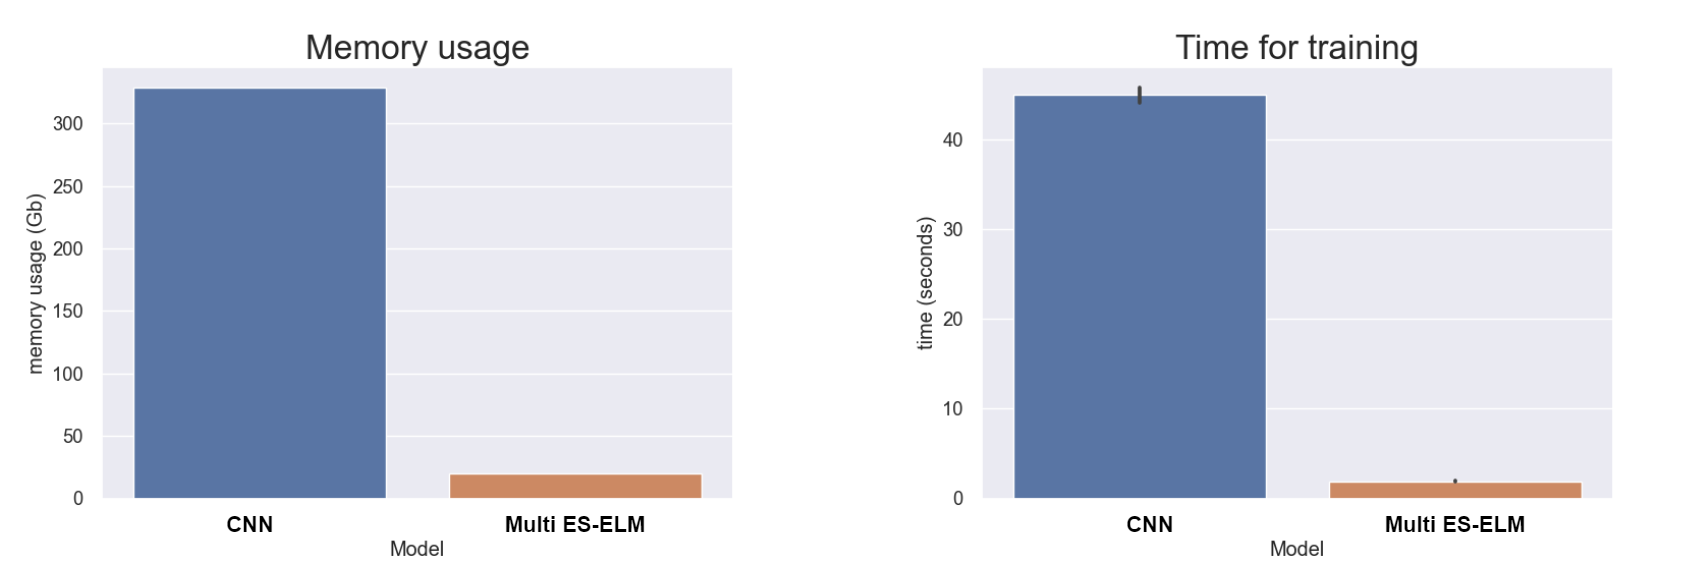
\includegraphics[width=\textwidth]{img/mem_time.png}
    \caption{memory and time for training usage}
    \label{fig:memetime}
\end{figure}

Figure \ref{fig:memetime} shows that the RC model can train extremely fast and is 23 times faster than the CNN model. Moreover, the memory usage for the training of the RC model is 16 times less than that of the CNN model.\\



\section{Conclusion}

The EEW system faces a significant hurdle. While its model effectively identifies seismic waves for alerts. However, the model in the system like a CNN consumes a lot of resources (computational time, and memory).
This research proposed an ESN model for predicting the earthquake's strong motion. The ESN model is one of reservoir computing that needs small resources to train and implement. The model can extract features from the initial P-wave like an RNN model but no need to train recurrent units. The prediction part is trained by an extreme learning machine that optimizes loss in just one short. 

The proposed model, the combination of ESN and ELM called Multi ES-ELM, contributes to using little time and low memory resources. Also, the Multi ES-ELM model can make performance close to the performance of the convolutional neural network model and uses resources less than the convolutional neural network model.

The proposed EEW models are very fast to train and require small resources. However, the proposed models are quietly sensitive to noise signals. The reason for the decrease is the models overfit with noise training data. 

In future work, to avoid this problem, in the future, we would like to investigate the other models or methods that help to denoise the signal before passing it through the EEW models.